\documentclass{article}

\usepackage[utf8]{inputenc}
\usepackage{url}
\usepackage{amsmath}
\usepackage{graphicx}
\usepackage{geometry}
\usepackage{ragged2e}

\geometry{
a4paper,
left=30mm,
right=20mm,
top=30mm,
bottom=20mm,
}

\renewcommand{\contentsname}{Sumário}
\renewcommand{\listfigurename}{Figuras}
\begin{document}

	\pagenumbering{gobble}
	\begin{center}

		{\LARGE Universidade Federal de Santa Catarina \par}
		\vspace {2cm}
		
		Ciências da Computação
		\vspace{2cm}

		Luca Fachini Campelli
		\vspace {4cm}

		\textbf{DESENVOLVIMENTO DE UMA APLICAÇÃO PARA COLETA DE DADOS \\
				E EMISSÃO DE PASSAPORTES ELETRÔNICOS NA PLATAFORMA JAVACARD}
		\vspace {10cm}
		
		Florianópolis/SC \\

		2018
	\end{center}

	\newpage
	\begin{center}
		Luca Fachini Campelli
		\vspace{2cm}
		
		\textbf{\large DESENVOLVIMENTO DE UMA APLICAÇÃO PARA COLETA DE DADOS \\
				E EMISSÃO DE PASSAPORTES ELETRÔNICOS NA PLATAFORMA JAVACARD}
		\vspace{2cm}

		\hfill \textbf{Trabalho de Conclusão de Curso \\}
		\hfill \textbf{para a graduação no curso de\\}
		\hfill \textbf{Ciências \hspace{18pt} da \hspace{18pt} Computação \\}
		\hfill \textbf{UFSC  \hspace{60pt}}

		\vspace{1cm}

		\hfill Florianópolis, 2018

	\end{center}

	\newpage

	\paragraph{\large Resumo (Melhorar)}
		\begin{justify}
			\hspace{2cm} Foi desenvolvido um software para computador capaz de coletar as informações do usuário, e emitir um passaporte eletrônico em um Javacard que segue o padrão ICAO 9303. Este cartão é munido de todas as informações necessárias para a verificação da identidade do usuário, incluindo informações biométricas como identificação facial, e digitais, juntamente com todos os mecanismos de segurança descritos pelo documento ICAO 9303.
	
	\vspace*{10px}
Palavras-chave: Javacard, Passaporte,JMRTD, Segurança, Passaporte-Eletrônico, e-Passport, SmartCard, JCOP
		\end{justify}


	\paragraph{\large Abstract}
		\begin{justify}

			\hspace{2cm} A computer software was developed capable of collecting user information, and emiting an electronic passport on a Javacard that follows the ICAO 9303 standard. This card posesses all required information to verify the user's identity, including biometrics such as face recognition and fingerprints, together with all security mecanisms described in the ICAO 9303 document.

	\vspace*{10px}
Key-Words: Javacard, Passaport,JMRTD, Security, Electronic-Passport, e-Passport, SmartCard, JCOP

		\end{justify}
	
	\newpage

	\tableofcontents
	\listoffigures
	\newpage

	\pagenumbering{arabic}

	\section{Introdução (Modificar, muito)}
		\begin{justify}
			
			\hspace{2cm} Quando começaram a ser utilizados, os passaportes funcionavam apenas por meio físico, na forma de uma caderneta ou documento escrito, com todas as informações sendo verificadas manualmente, comparando as informações com o outros papéis, ou com um sistema eletrônico. Isto acarreta em uma passagem mais lenta pelo controle e abre muitas brechas para erros e falsificações passarem pelos vigías. Várias formas de prevenir falsificações como marcas d’água, padrões de impressão e manufatura do papel foram utilizadas, porém a inovação mais impactante e discutida foi a inserção de um chip dentro do passaporte. Embora várias informações possam ainda ser verificadas visualmente, mais ainda podem ser verificadas por meio eletrônico com o chip interno do passaporte, e mais rapidamente, diminuindo o risco de fraude. Este chip pode guardar as informações biométricas do dono, junto com as informações visuais, e ainda mais importante, possuindo diversos protocolos de segurança para garantir a autenticidade dos dados conferidos \cite{PASSPORTWIKI}\cite{HOWPASSPORT}.
			\hspace*{2cm} Diversos softwares existem para a leitura de passportes e em sua maioria se utilizam da biblioteca JMRTD\cite{JMRTD} como base para seu funcionamento, poucos utilizam outras bibliotecas de código fechado, como o software de leitura de chips NFC da empresa InnoValor\cite{INNOVALOR}, mas não foi possível encontrar o software utilizado por aeroportos para a verificação de passaportes. Apenas um software foi encontrado que efetivamente recolha dados e emita um passaporte sendo este uma versão antiga da biblioteca JMRTD que possuía um aplicativo standalone para emissão e leitura de passaportes eletrônicos, este que foi descontinuado da versão 0.4.9 para a versão 0.5, mantendo o pacote apenas como uma biblioteca de leitura. 
			\hspace*{2cm} Desta forma para cumprir os requisitos de recolher as informações do usuário e emitir um passaporte válido de acordo com o padrão ICAO9303, será utilizado esta parte da versão 0.4.9 do aplicativo para a personalização do cartão.

			
		\end{justify}

	\subsection{Objetivos}
		\begin{justify}
				
				\hspace{2cm}O objetivo principal é a criação do sistema de coleta de dados e emissão de um passaporte eletrônico em um cartão Javacard, onde os dados sejam armazenados depois possam ser extraídos e validados em qualquer tipo de máquina que possua este sistema.\\
				\hspace*{2cm}Os objetivos específicos se dão por:\\
					\hspace*{3cm}1.Coleta dos dados básicos do usuário\cite{SASSO}\\
					\hspace*{3cm}2.Coleta da foto do usuário e extração dos dados faciais da foto\cite{ISO}\cite{ICAO}.\\
					\hspace*{3cm}3.Coleta dos dados biométricos como digital e íris.\\
					\hspace*{3cm}4.Ter o cartão preenchido e que cumpra as especificações do padrão ICAO9303.\cite{ICAO}\\
					\hspace*{3cm}5.Ter o programa que colete os dados do usuário de forma rápida e fácil.\\
				 \hspace*{2cm}Ao final do projeto espera-se ter concluído a criação de um sistema que colete os dados do usuário, armazenando-os no banco de dados e no cartão, e que emita o cartão conforme as especificações ditadas no padrão ICAO9303

			
		\end{justify}

	\section {Conceitos Básicos}
		\subsection{O que é segurança computacional? [\cite{STALLINS} - cap 1]}
			\begin{justify}
			
				\hspace{2cm} Segurança computacional engloba todas as áres de pesquisa relacionadas a manter algum tipo de informação segura, seja ela uma senha, listas de cadastros, um banco de dados, documentos ou uma receita de bolo. As pesquisas relacionadas a segurança computacional, trabalham para proteger estas informaçôes de pessoas que as poderiam utilizar para maus fins, seja impedindo que elas sejam obtidas ou entendidas por outras pessoas, ou garantindo que uma informação não foi alterada antes de ser entregue ao destinatário. As próximas seções deste documento explicam certos campos desta área que serão tratados.
			
			\end{justify}

		\subsection{Criptografia Simétrica e Assimétrica [\cite{STALLINS} -parte 1 - parte 2]}
			\begin{justify}
			

	 			\hspace{2cm} É possível cifrar a informação para que apenas quem possua a chave da cifra possa acessa-la. O ato de embaralhar o significado da mensagem se chama cifrar, e o inverso, decifrar. Para tal, utiliza-se algum tipo de algoritmo que, em conjunto com uma chave, seja capaz de mascarar a informação original e que seja reversível, para que com o uso da chave, se possa desfazer a criptografia e acessar o conteúdo original da mensagem. Nesta área existem dois tipos de protocolos para cifrar mensagens: a criptografia Simétrica e a Assimétrica. \\
				\hspace*{2cm}Na criptografia simétrica, uma única chave é utilizada por ambas as partes, para cifrar e decifrar a mensagem. Na criptografia assimétrica, são utilizadas duas chaves distintas, uma pública e uma privada. Ambas podem ser usadas para cifrar, porém o que uma cifrar, somente poderá ser decifrado pela outra. Devido às dificuldades de se utilizar este protocolo ele é mais utilizado para certificações digitais.
					
			\end{justify}

		\subsection{Função Hash - SHA [\cite{STALLINS} - cap 11 - pg313]}
			\begin{justify}
			

				\hspace{2cm} Esta função é amplamente utilizada para garantia de consistência tanto em criptografia quanto em várias outras áreas. Esta função funciona embaralhando os bits de uma mensagem à um ponto que seja impossível inverter o processo. Ela aceita uma mensagem de qualquer tamanho, porém sempre retornará uma cadeia de bytes de tamanho fixo, não importando qual seja a entrada. Porém a maior característica desta função está no fato de que para duas entradas distintas x e y quaisquer, o resultado da função sempre será diferente para os dois. Desta forma, é possível se checar a integridade de uma mensagem, aplicando a função hash sobre ela antes de ser enviada, e depois de recebida, e comparando as saídas, pois se a mensagem foi alterada, por menor que seja a alteração, os dois resultados da função serão completamente diferentes. O algoritmo mais utilizado para esta função é o SHA 2 - Secure Hash Algorithm 2(Algoritmo de Hash Seguro 2), projetado pela NSA, e possui seis versões diferentes, onde a mudança principal está no número de bits que eles retornam: SHA-224, SHA-256, SHA-384, SHA-512, SHA-512/224, SHA-512/256. 
			
			\end{justify}

		\subsection{Assinaturas Digitais[\cite{STALLINS} - cap 13.1 - pg 395]}
			\begin{justify}
			

				\hspace{2cm}A confiança entre duas partes de uma troca de mensagens pode não ser suficiente para que informação sensível seja transferida. Uma parte “A” pode forjar uma mensagem alegando ter sido enviada pela parte “B”, ou “B” pode simplesmente negar ter enviado qualquer mensagem, mesmo que o tenha. Desta forma, um meio de proteger âmbas as partes contra fraude mútua são as assinaturas digitais.
		Uma assinatura digital consiste normalmente da própria mensagem "M", passada pela função hash e cifrada com a chave privada do remetente, concatenada ao fim da mensagem. Ao ser recebida esta assinatura pode ser verificada, removendo-a da mensagem, decifrando-a com a chave pública do remetente e comparando-a com a hash da mensagem recebida. Sendo assim duas afirmações podem ser concluídas: apenas o remetente pode ter enviado a mensagem, pois apenas a sua chave privada pode ser decifrada com sua chave pública, e a mensagem não foi alterada durante seu trajeto, pois as hash's coicidem.
			
			
			\end{justify}


		\begin{figure}[hb!]
			\centering
			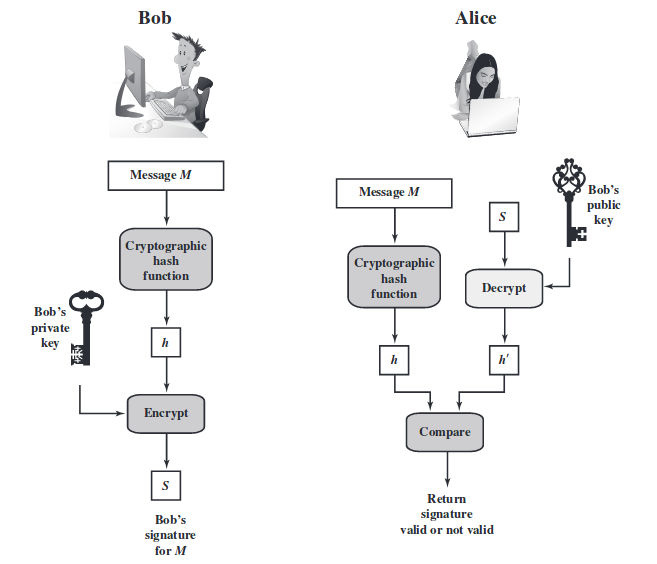
\includegraphics[width=250px]{AssinaturaDigital.png}
			\caption{Descrição simplificada do funcionamento de uma assinatura digital.}
			\label{fig:digiSign}

		\end{figure}

		\subsection{Certificados Digitais[\cite{STALLINS} - cap 14.4 - pg 435]}
			\begin{justify}
			
				
					\hspace{2cm}Certificados digitais são documentos eletrônicos que garantem a autenticidade de um certo elemento. Este que pode ser uma entidade, um site da internet ou um terminal de cartões. Um certificado é composto de algumas informações da entidade,  a chave pública da entidade, e uma assinatura digital sobre o certificado. Dependendo do tipo de certificado, esta assinatura adicionada ao final do documento é cifrada ou com a chave privada de quem o criou, denominado de certificado auto-assinado, ou com a chave privada de uma autoridade certificadora (CA - Certificate Authority). \\

			
			\end{justify}

    
	\section{O Documento ICAO 9303\cite{ICAO} - Remover Talvez?}
		\begin{justify}
			
				\hspace*{2cm} O documento ICAO 9303 é o documento emitido que regulamenta passaportes eletrônicos, e é o padrão utilizado para toda formatação de passaportes eletrônicos. ICAO é uma sigla para “International Civil Aviation Organization”, que é uma agência especializada das Nações Unidas. Foi estabelecida em 1944 para gerenciar a admnistração e governância da Convenção de Aviação Civil Internacional (Convenção de Chicago). \\
    			\hspace*{2cm} O documento é escrito em 12 partes, cada uma descreve um aspecto sobre como um passaporte eletrônico deve ser desenvolvido, a primeira parte dando uma introdução sobre o as características de um passaporte eletrônico, e definindo siglas e acrônimos para os documentos seguintes.\\
    			\hspace*{2cm} A segunda parte da especificações sobre a segurança física do cartão, desde o design interno, quanto a produção, transporte e criação do cartão. \\
				\hspace*{2cm} A terceira parte especifica as características sobre a apresentação de todos os tipos de passaporte, como fonte, linguagem, campos de preenchimento e representação das informações. \\
				\hspace*{2cm} A quarta parte específica como os dados para passaportes legíveis por máquina, que possuem forma de livreto como são hoje, mostrando dimensões e formatos dos campos, também chamado de tipo TD3. \\
				\hspace*{2cm} A quinta parte especifica como deve ser o layout dos dados para passaportes do tipo cartão plástico impresso, chamado TD1. Este cartão possui uma zona legível por máquina (MRZ), que possui os dados básicos de seu portador, formatados para mais fácil leitura humana e por máquina, impresso em seu exterior junto com todas as outras informações no verso, e uma imagem do portador.\\
				\hspace*{2cm} A sexta parte se assemelha à quinta, pois descreve as características de cartões do tipo TD2, que possuem de diferente do tipo TD1 apenas suas dimensões, tendo todas as informações necessárias em um lado do cartão, permitindo informações opcionais serem adicionadas ao verso.\\
				\hspace*{2cm} A sétima parte se refere à vistos legíveis por máquina. Estes se assemelham aos tipos de passaportes TD1 e TD2, porém possuem as informações referentes aos vistos.\\
				\hspace*{2cm} A oitava parte não foi preenchida ainda, e é mantida reservada para uso futuro.\\
				\hspace*{2cm} A nona parte fala sobre como se deve dispor das informações biométricas do portador do passaporte, formatos e dados, tomando como principal a identificação facial da pessoa, e como identificações secundárias as digitais e íris.\\
				\hspace*{2cm} A décima parte especifica a estrutura logica de dados (LDS) do cartão, e como se deve armazenar os dados biométricos dentro do cartão.\\
				\hspace*{2cm} A décima primeira parte especifica como funcionam os protocolos de segurança necessários à comunicação do cartão e obtenção dos dados biométricos para verificação da identidade da pessoa.\\
				\hspace*{2cm} Por último a décima segunda parte especifica o funcionamento de todas as assinaturas digitais necessárias à certificação do cartão via chaves públicas, e sua infra-estrutura.\\

		\end{justify}

	\section{Javacard\cite{JAVACHEN}}
		\begin{justify}
			

				\hspace{2cm} O Javacard é um cartão eletrônico que possui dois componentes principais, Um chip de contato e um processador interno. Este chip de contato se faz presente do lado externo do cartão, da mesma forma que cartões de crédito ou débito modernos, e cuida da comunicação do cartão com a leitora. O processador interno funciona como um computador, ele roda um sistema operacional Java, o que torna este cartão um Javacard. Ele também possui uma memória interna capaz de armazenar dados. O que diferencia este cartão de cartões de crédito por exemplo, é o fato de o cartão possuir um máquina virtual Java (JVM) instalada. A JVM faz possível o cartão possuir aplicativos em sua memória, e dependendo do programa que os acessar, pode escolher qual deles executar. Estes aplicativos conversam com o terminal por meio de mensagens, chamadas APDU's, que são em sua maioria padronizadas em alguns formatos específicos. O Chip de contato fornece energia e faz a comunicação entre a leitora ou terminal e o processador. Estes cartões possuem diversos mecanismos de segurança embutidos na própria JVM, os aplicativos rodam isolados uns dos outros, portanto os dados de um aplicativo nunca poderão serem lidos por outro. Os cartões também suportam funções de criptografia, que dependem dos aplicativos para serem utilizadas.

			
		\end{justify}


	\section{O aplicativo e sua estrutura lógica de dados - Remover talvez?}
		\begin{justify}

			\hspace{2cm} A biblioteca JMRTD possui consigo um aplicativo a ser instalado e executado no cartão para o funcionamento da biblioteca\cite{SASSO}. Este aplicativo foi feito juntamente com a biblioteca no padrão ICAO9303, portanto ele pode ser lido inclusive por outras bibliotecas que implementem o padrão. Este aplictivo tem como função armazenar todas as informações referentes a um passaporte, e portanto possui uma estrutura de dados lógica interna descrita pelo padrão ICAO9303:\\
			
			\hspace*{1.5cm} DG 1 — Informação da Zona Legível por Máquina\\
			\hspace*{2cm} DG 2 — Características Faciais (Foto)\\
			\hspace*{2cm} DG 3 — Informações de identificação adicionais (Digitais)*\\
			\hspace*{2cm} DG 4 — Informações de identificação adicionais (Iris)*\\
			\hspace*{2cm} DG 5 — Fotografia impressa na frente do cartão*\\
			\hspace*{2cm} DG 6 — Reservado para uso futuro*\\
			\hspace*{2cm} DG 7 — Assinatura escrita digitalizada*\\
			\hspace*{2cm} DG 8 — Características de dados* **\\
			\hspace*{2cm} DG 9 — Características estruturais* **\\
			\hspace*{2cm} DG 10 — Características substanciais*\\
			\hspace*{2cm} DG 11 — Detalhes pessoais adicionais*\\
			\hspace*{2cm} DG 12 — Detalhes do documento adicionais*\\
			\hspace*{2cm} DG 13 — Detalhes opcionais*\\
			\hspace*{2cm} DG 14 — Informações da chave pública para Autenticação Passiva***\\
			\hspace*{2cm} DG 15 — Informações da chave pública para Autenticação Ativa***\\
			\hspace*{2cm} DG 16 — Pessoas para contato*\\

			\hspace*{2cm} * - Opcional\\
			\hspace*{2cm} ** - Ainda não definido, estrutura geral que acomoda qualquer tipo de dados\\
			\hspace*{2cm} *** - Condicional, apenas se suportado\\
			
			\hspace*{2cm}Além destes existem mais dois arquivos que não armazenam dados do usuário mas sim dados do cartão, estes são: COM e SOD.\\
			\hspace*{2cm} O arquivo COM, ou Arquivo de Cabeçalho e de Presença de Grupos de Dados, possui a função de armazenar a presença dos arquivos de dados, ou seja, quais arquivos estão presentes no cartão, e informações de versionamento do sistema de arquivos do cartão. \\
			\hspace*{2cm} O arquivo SOD, ou Document Security Object - Objeto de Segurança do Documento, possui a função de armazenar o resultado da função hash de cada arquivo, ou seja, no processo de emissão do cartão, cada arquivo é passado também pela função hash, e seu resultado é armazenado dentro do arquivo SOD. Ele também armazena todas as informações de segurança do cartão como os algoritmos utilizados para a função hash e criptografia.
			\hspace*{2cm} O cartão possui também uma zona que é ilegível por meios externos, informações sensíveis a criptografia como chaves privadas são armazenadas ali na sua criação, e depois só podem ser lidas pelo próprio cartão.
		\end{justify}

	\section{As bibliotecas utilizadas}
		\begin{justify}
			 
		\hspace{2cm}O sistema principal será desenvolvido na linguagem de programação Java, porém algumas das bibliotecas escolhidas foram escritas na linguagem de programação C ou C++ exigindo a utilização da Interface Nativa Java (JNI) para sua utilização.\\
		
        \hspace*{2cm}JMRTD\cite{JMRTD}\\
    \hspace*{2cm}Java Machine Readable Travel Documents: é uma biblioteca para a criação, edição, e aferição de passaportes eletônicos escrita na linguagem de programação Java. Ela foi desenvolvida juntamente com a biblioteca Scuba, que a complementa. Ela possui a capacidade de criar, e editar novos passaportes, além que resgatar as informações de um passaporte pronto. \\
        
		\hspace*{2cm}SCUBA\cite{SCUBA}\\
    \hspace*{2cm}Smart Card Utilities for Better Access: é uma biblioteca para a comunicação com cartões eletrônicos da plataforma javacard, escrita na linguagem de programação Java. Ela faz a ponte entre o JMRTD e o javacard possuindo a capacidade de transmitir mensagens e prover a comunicação com os cartões.\\
		
        \hspace*{2cm}STASM\cite{STASM}\\
    \hspace*{2cm}Active Shape Models with STASM: é uma biblioteca de reconhecimento facial escrita na linguagem de progrmação C++. Ela se utiliza de modelos de formas para reconhecer um rosto em uma foto e retirar os pontos de referência do rosto para que depois seja feito o reconhecimento da pessoa, fazendo uso da biblioteca Open-CV. Possui a maioria dos pontos de reconhecimento parecida com o padrão ISO\cite{ISO}, e foi escolhida por ser de fácil utilização e possuir uma extensa documentação com exemplos mínimos disponíveis, facilitando a sua compreensão, além de ser complementar à biblioteca Open-CV.\\
		
        \hspace*{2cm}LIBFPRINT\cite{PRINT}\\
    \hspace*{2cm}É uma biblioteca de coleção e verificação de digitais biométricas escrita na linguagem de programação C. Ela provê funções para se coletar uma digital e guardá-la como uma imagem, e depois extrair as minutas desta imagem para que se compare com uma digital recém tirada. Foi escolhida por ter uma documentação extensa, exemplos mínimos e ter sido recomendada pelo orientador deste projeto.\\
		
        \hspace*{2cm}OPEN-CV\cite{OPENCV}\\
    \hspace*{2cm}Open Source Computer Vision Library: é uma biblioteca para manipulação de imagens e visão computacional escrita na linguagem de programação C++ e Java. Ela possui funcionalidades para conversão de imagens, e acessar a câmera do dispositivo para tirar fotos ou videos. Ela também provê visão computacional, permitindo identificar formas e rostos na imagem. A biblioteca Stasm amplia a funcionalidade para rostos, detectando mais pontos de interesse no rosto da pessoa, e foi escolhida por ser a mais bem recomendada biblioteca de manipulação de imagens e visão computacional, com relação a sua utilização.\\
		
        \hspace*{2cm}EJBCA\cite{EJBCA}\\
    \hspace*{2cm}Open Source PKI Certificate Authority: é uma biblioteca para criação e manejo de certificados digitais auto-assinados escrita na linguagem de programação Java. É necessária para o funcionamento da biblioteca JMRTD, para criação dos certificados verificáveis por cartão (CVC), necessários para a execução dos protocolos de segurança do cartão.\\
		
        \hspace*{2cm}BOUNCYCASTLE\cite{BOUNCYCASTLE}\\
    \hspace*{2cm}Bouncy Castle Security Provider: é um provedor de segurança, uma biblioteca que possui funções criptograficas e de geração e acordo de chaves para criptografia escrita na linguagem de programação Java. Toda a segurança da biblioteca do JMRTD é feita com ele, portanto por motivos de compatibilidade foi-se utilizado o bouncycastle como provedor para o sistema final.\\

			
		\end{justify}


	\section{Desenvolvimento - Reescrever?}
		\begin{justify}
			
		\hspace{2cm}O projeto foi desenvolvido tendo como base o aplicativo JMRTD\cite{JMRTD}, que engloba uma Biblioteca Java e um Applet, para que seja criado um aplicativo que emita os passaportes, e que possa ser expandido caso haja a necessidade, para englobar mais documentos e não só o passaporte.\\
		\hspace*{2cm}Foi feita uma extensa pesquisa sobre os documentos ICAO 9303\cite{ICAO}, e a documentação da biblioteca JMRTD para se iniciar o projeto.\\
		\hspace*{2cm}O programa foi desenvolvido com a linguagem de programação Java, utilizando o sistema JNI para a integração de bibliotecas que existem somente em C e C++, e as bibliotecas JMRTD, como a biblioteca principal para a construção do cartão, BouncyCastle\cite{BOUNCYCASTLE} e EJBCA\cite{EJBCA} como provedores de segurança e certificação, libfprint\cite{PRINT} para a coleta das digitais biométricas, Stasm\cite{STASM} para o reconhecimento facial, e OpenCV\cite{OPENCV} para processamento de imagem.\\
		\hspace*{2cm}Utilizando uma parte do código da versão 0.4.9 da biblioteca JMRTD, é possível enviar informações para o cartão, desta forma pode-se fácilmente coletar e enviar as informações à respeito do MRZ. A biblioteca OpenCV foi usada para o processamento da foto da pessoa, e possui funções para tirar a foto com a camera da máquina. Com a biblioteca Stasm, se pode retirar os pontos faciais da pessoa, e depois tratá-los para se adequarem ao padrão ICAO. Foi necessário utilizar a API nativa do java para integrar as bibliotecas Stasm e libfprint ao projeto, pois elas existem apenas em C. Com a biblioteca libfprint foi possível a extração da digital para sua inserção.

		\end{justify}


	\subsection{Os protocolos de segurança}
		\begin{justify}
			\hspace{2cm}Para o acesso as informações do cartão diversos protocolos de segurança devem ser efetuados para garantir a troca segura de mensagens entre o terminal e o cartão, e ter a certeza de que o terminal e o cartão não foram adulterados de alguma maneira. Estes protocolos devem ser corretamente configurados durante a criação do cartão para que garantam a segurança das informações que nele estão guardadas. Todos os protocolos estão completamente descritos no documento ICAO 9303 parte 11\\

			\hspace*{2cm} BAC - Basic Access Control - Controle de Acesso Básico\\
			\hspace*{2cm} Antes de fazer qualquer tipo de operação no cartão, deve-se efetuar este protocolo. Ele utiliza as informações do número do documento, data de nascimento e de validade do cartão para criar chaves simétricas seguras para a troca de mensagens entre o terminal e o cartão criando assim um canal seguro de comunicação. Esta informação estará impressa na frente do cartão, e portanto a execução com sucesso deste protocolo não só garante um canal de comunicação seguro, mas também confirma que as informações impressas batem com as armazenadas no cartão.\\
			
			\hspace*{2cm} PA - Passive Authentication - Autenticação Passiva\\
			\hspace*{2cm} Este protocolo faz uso dos arquivos COM e SOD para seu funcionamento. O arquivo SOD armazena a hash de cada Grupo de Dados presente no cartão, e o arquivo COM indica sua presença. Desta forma o protocolo se inicia verificando se para cada arquivo cuja presença esteja indicada em COM, incluindo o próprio arquivo COM, se sua hash coincide com a hash armazenada em SOD. Se todas coincidirem então nenhum arquivo foi alterado desde a fabricação do cartão.\\
			\hspace*{2cm} O segundo passo consiste em utilizar o certificado de assinatura encontrado no SOD, construindo uma corrente de certificação até um certificado assinado por uma CA reconhecida, e garantindo que cada certificado da corrente seja válido. Passados por estes dois passos então se pode confirmar que os dados do cartão são válidos e não foram alterados.\\
			
			\hspace*{2cm} AA - Active Authentication - Autenticação Ativa\\
			\hspace*{2cm} Este protocolo deve ser feito após o PA, pois ele confirma que o SOD foi lido de um cartão com um chip válido. Ele consiste em uma troca de mensagens de desafio-resposta onde a aplicação envia uma mensagem ao cartão e este responde com esta mensagem cifrada pela chave privada do cartão. A aplicação então decifra utilizando a chave pública armazenada no arquivo DG15 e, caso a resposta coincida com a mensagem enviada, então o chip não foi adulterado, já que a chave privada interna do cartão, inacessível externamente, é o par da chave pública gravada no arquivo DG15.\\
			
			\hspace*{2cm} EAC - Extended Access Control - Controle de Acesso Extendido\\
			\hspace*{2cm} Este protocolo deve ser feito após o BAC e é necessário para se obter acesso as biometrias adicionais do cartão. Ele consiste em autenticar o terminal para o cartão, e o cartão para o terminal em duas etapas, utilizando-se de um par de chaves assimétricas. Ao término do protocolo um canal de comunicação de maior segurança entre o cartão e o terminal é gerado, e o acesso às biometrias adicionais é liberado.
			
		\end{justify}

	\subsection{Funcionamento}
		\begin{justify}
			\hspace{2cm} O aplicativo desenvolvido possui duas funções, coletar as informações do usuário e com ela gerar um novo passaporte válido, e verificar se as informações coletadas estão devidamente inseridas no cartão. A parte da verificação de identidade do proprietário não faz jús ao escopo deste trabalho. O aplicativo possui as funções de retirar uma foto da pessoa, e de coletar todas as suas digitais. O aplicativo também necessita de certificados digitais e pares de chaves para que os protocolos de segurança possam ser executados.
			
		\end{justify}

	\section{}
		\begin{justify}
			
			
		\end{justify}

\begingroup
	\section{Referências}
		\renewcommand{\section}[2]{}
		
		\bibliography{TCC}
		\bibliographystyle{plain}
		
\endgroup
\end{document}
